\begin{enumerate}[label=\thechapter.\arabic*,ref=\thechapter.\theenumi]

\item The damping ratio and undamped natural frequency of a closed loop system as
shown in the figure, are denoted as $\zeta$ and $\omega_n$, respectively. The values of $\zeta$ and $\omega_n$
are 
\begin{figure}[!ht]
\centering
\begin{center}
\includegraphics[width=\columnwidth]{2022/EE/39/figs/question.jpg}
\end{center}
%\caption{Diagram for GATE ME Question 30}
\end{figure}
\begin{enumerate}
    \item $\zeta = 0.5$ and $\omega_n = 10$ rad/s
    \item $\zeta = 0.1$ and $\omega_n = 10$ rad/s
    \item $\zeta = 0.707$ and $\omega_n = 10$ rad/s
    \item $\zeta = 0.707$ and $\omega_n = 100$ rad/s
\end{enumerate}
\hfill(GATE EE 2022)
\solution
\iffalse
\let\negmedspace\undefined
\let\negthickspace\undefined
\documentclass[journal,12pt,twocolumn]{IEEEtran}
\usepackage{cite}
\usepackage{amsmath,amssymb,amsfonts,amsthm}
\usepackage{algorithmic}
\usepackage{graphicx}
\usepackage{textcomp}
\usepackage{xcolor}
\usepackage{txfonts}
\usepackage{listings}
\usepackage{enumitem}
\usepackage{mathtools}
\usepackage{gensymb}
\usepackage{comment}
\usepackage[breaklinks=true]{hyperref}
\usepackage{tkz-euclide} 
\usepackage{listings}
\usepackage{gvv}                                        
\def\inputGnumericTable{}                                 
\usepackage[latin1]{inputenc}                                
\usepackage{color}                                            
\usepackage{array}                                            
\usepackage{longtable}                                       
\usepackage{calc}                                             
\usepackage{multirow}                                         
\usepackage{hhline}                                           
\usepackage{ifthen}                                           
\usepackage{lscape}
\usepackage{placeins}
\usepackage{xparse}


\newtheorem{theorem}{Theorem}[section]
\newtheorem{problem}{Problem}
\newtheorem{proposition}{Proposition}[section]
\newtheorem{lemma}{Lemma}[section]
\newtheorem{corollary}[theorem]{Corollary}
\newtheorem{example}{Example}[section]
\newtheorem{definition}[problem]{Definition}
\newcommand{\BEQA}{\begin{eqnarray}}
\newcommand{\EEQA}{\end{eqnarray}}
\newcommand{\define}{\stackrel{\triangle}{=}}
\theoremstyle{remark}
\newtheorem{rem}{Remark}

\graphicspath{ {./figs/} } 

\begin{document}

\bibliographystyle{IEEEtran}
\vspace{3cm}

\Large\title{GATE 2022 EE 39}
\large\author{EE23BTECH11032 - Kaustubh Parag Khachane $^{*}$% <-this % stops a space
}
\maketitle
\newpage
\bigskip

\renewcommand{\thefigure}{\theenumi}
\renewcommand{\thetable}{\theenumi}
\large\textbf{Question GATE 22 EE 39} :\\
The damping ratio and undamped natural frequency of a closed loop system as
shown in the figure, are denoted as $\zeta$ and $\omega_n$, respectively. The values of $\zeta$ and $\omega_n$
are 
\begin{figure}[!ht]
\centering
\begin{center}
\includegraphics[width=\columnwidth]{question}
\end{center}
%\caption{Diagram for GATE ME Question 30}
\end{figure}
\begin{enumerate}
    \item $\zeta = 0.5$ and $\omega_n = 10$ rad/s
    \item $\zeta = 0.1$ and $\omega_n = 10$ rad/s
    \item $\zeta = 0.707$ and $\omega_n = 10$ rad/s
    \item $\zeta = 0.707$ and $\omega_n = 100$ rad/s
\end{enumerate}
\hfill(GATE EE 2022)\\
\solution\\
\fi
\begin{table}[!ht] 
\centering
\setlength{\extrarowheight}{8pt}
\begin{tabular}{|l|l|l|}
    \hline
    \textbf{Parameter} & \textbf{Description} & \textbf{Values}\\
    \hline
     m & load of system &  \\
    \hline
     k & stiffness of system &  \\
    \hline
     $\omega_n$ & Natural frequency & $\sqrt{\frac{k}{m}}$ \\
    \hline
    $\zeta$ & Damping ratio & $\frac{c}{2m\omega_n}$ \\
    \hline
     y\brak{t} & Output of system & \\
    \hline
     x\brak{t} & Input to the system & \\
    \hline
     c & Damping coefficient & \\
    \hline
    T\brak{s} & Transfer function of system & $\frac{Y\brak{s}}{R\brak{s}}$\\
    \hline
  \end{tabular}
  \vspace{4mm}
 \caption{Parameter Table}
 \label{tab:table0_ee_22_39}
\end{table}

We will use Mason's Gain Formula to calculate the transfer function of this system. First converting the given diagram to a signal flow graph :

\begin{figure}[!ht]
\centering
\resizebox{0.5\textwidth}{!}{%
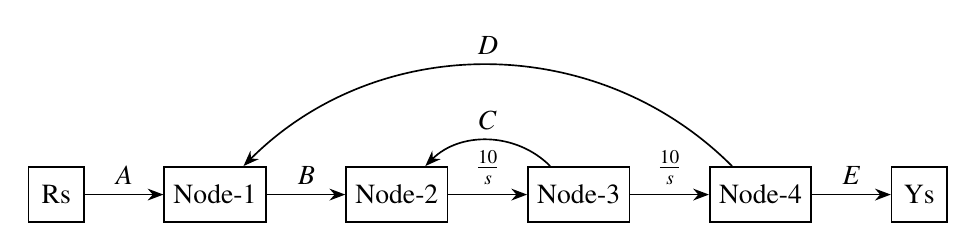
\begin{tikzpicture}[>=Stealth,auto,node distance=1cm,semithick]
  \tikzstyle{block}=[draw, fill=white, rectangle, minimum height=2em, minimum width=2em]
  
  \node [block] (input) {R\brak{s}};
  \node [block, right=of input] (filter) {Node-1};
  \node [block, right=of filter] (D) {Node-2};
  \node [block, right=of D] (E) {Node-3};
  \node [block, right=of E] (F) {Node-4};
  \node [block, right=of F] (output) {Y\brak{s}};
  
  \draw [->] (input) -- node {$A$} (filter);
  \draw [->] (filter) -- node {$B$} (D);
  \draw [->] (D) -- node {$\frac{10}{s}$} (E);
  \draw [->] (E) -- node {$\frac{10}{s}$} (F);
  \draw [->] (F) -- node {$E$} (output);
  
  % Backward loops
  \draw [->] (E) edge [bend right=45] node[above] {$C$} (D);
  \draw [->] (F) edge [bend right=45] node[above] {$D$} (filter);
\end{tikzpicture}%
}
\caption{Signal Flow Diagram}
\label{fig:your_label}
\end{figure}


Mason's Gain Formula is given by :
\begin{align}
    H\brak{s} = \sum_{i=1}^{N}\brak{\frac{P_i \Delta_i}{\Delta}} \label{eq:eq1_ee39}
\end{align}
\begin{table}[!ht] 
\centering
\setlength{\extrarowheight}{8pt}
\begin{tabular}{|l|l|}
    \hline
    \textbf{Parameter} & \textbf{Description}\\
    \hline
     N & Number of forward paths \\\hline
     L & Number of loops\\\hline
     $P_k$ & Forward path gain of $k^{th}$ path\\\hline
     $\Delta_k$ & Associated path factor \\\hline
     $\Delta$ & Determinant of the graph \\\hline
  \end{tabular}
  \vspace{4mm}
 \caption{Parameter Table - Mason's Gain Law}
 \label{tab:table1_ee_22_39}
\end{table}

\begin{table}[!ht] 
\centering
\setlength{\extrarowheight}{8pt}
\begin{tabular}{|l|l|}
    \hline
    \textbf{Parameter} & \textbf{Formula}\\
    \hline
     $\Delta$ & 1 + $\sum_{k=1}^{L}\brak{\brak{-1}^k\text{Product of gain of groups of k isolated loops}}$ \\\hline
     $\Delta_k$ & $\Delta$ part of graph that is not touching $k^{th}$ forward path \\\hline
  \end{tabular}
  \vspace{4mm}
 \caption{Formula Table - Mason's Gain Law}
 \label{tab:table2_ee_22_39}
\end{table}

This signal flow graph has only one forward path whose gain is given by :
\begin{align}
    P_1 &= \frac{10}{s} \frac{10}{s}\\
    &= \frac{100}{s^2}
\end{align}
The loop gain for loop between Node-2 and Node-3 is :
\begin{align}
    L_1 &= \frac{10}{s}\brak{-1}\\
    &= -\frac{10}{s}
\end{align}
The loop gain for loop between Node-1 and Node-4 is :
\begin{align}
    L_1 &= \frac{10}{s}\frac{10}{s}\brak{-1}\\
    &= -\frac{100}{s^2}
\end{align}
Using \tabref{tab:table2_ee_22_39}, $\Delta$ is :
\begin{align}
    \Delta &= 1 - \brak{-\frac{10}{s} - \frac{100}{s^2}}\\
    &= 1 + \frac{10}{s} + \frac{100}{s^2}
\end{align}
There are no two isolated loops available. Hence all further terms will b zero.\\
As both the loops are in contact with the only forward path,
\begin{align}
    \Delta_1 = 1
\end{align}
Using equation \eqref{eq:eq1_ee39} :
\begin{align}
    H\brak{s} &= \frac{\frac{100}{s^2}}{1 + \frac{10}{s} + \frac{100}{s^2}} \\
    &= \frac{100}{s^2 + 10s + 100}\label{eq:eq2_ee39}
\end{align}
Referring to \tabref{tab:table0_ee_22_39}, the general equation of the damping system is second order and can be written as :
\begin{align}
    m\ddot{y}(t) + c\dot{y}(t) + ky(t) = x(t)
\end{align}
Take the Laplace transform and solve for $\frac{Y\brak{s}}{X\brak{s}}$ :
\begin{align}
    \frac{Y\brak{s}}{X\brak{s}} &= \frac{\omega_n^2}{s^2 + 2\zeta\omega_n s + \omega_n^2}\\
\implies H\brak{s} &= \frac{\omega_n^2}{s^2 + 2\zeta\omega_n s + \omega_n^2} \label{eq:eq3_ee39}
\end{align}
Comparing equations \eqref{eq:eq2_ee39} and \eqref{eq:eq3_ee39} ,
\begin{align}
    \omega_n ^2 &= 100\\
    \implies \omega_n &= 10 \text{ rad/s} \label{eq:eq4_ee39}\\
    2\zeta \omega_n &= 10\\
    \implies \zeta &= 0.5
\end{align}
\begin{figure}[!ht]
\centering
\begin{center}
\includegraphics[width=\columnwidth]{2022/EE/39/figs/Figure_1.jpg}
\end{center}
\caption{Magnitude plot}
\end{figure}
\begin{figure}[!ht]
\centering
\begin{center}
\includegraphics[width=\columnwidth]{2022/EE/39/figs/Figure_2.jpg}
\end{center}
\caption{Phase plot}
\end{figure}

\newpage
\item In the block diagram shown in the figure, the transfer function $G=\frac{K}{\tau s+1}$ with $K>0$ and $\tau>0$. The maximum value of $K$ below which the system remains stable is \rule{1cm}{0.15mm}(rounded off to two decimal places) \hfill (GATE CH 2022) 
\begin{figure}[htbp] 
\includegraphics[width=\columnwidth]{2022/CH/58/figs/question.jpg} 
\end{figure}\\ 
\solution 
\input{2022/CH/58/ch_58.tex} 
\newpage

\item
A series RLC circuit is connected to 220 V, 50 Hz supply. For a fixed a value of R and C, the inductor L is varied to deliver the maximum current. This value 0.4A and the corresponding potential drop across the capacitor is 330 V. The value of the inductor L is ? (Rounded off to two decimal places).
\hfill{(GATE BM 2022)}\\
 \solution
 \iffalse
\let\negmedspace\undefined
\let\negthickspace\undefined
\documentclass[journal,12pt,onecolumn]{IEEEtran}
\usepackage{cite}
\usepackage{amsmath,amssymb,amsfonts,amsthm}
\usepackage{algorithmic}
\usepackage{graphicx}
\usepackage{textcomp}
\usepackage{xcolor}
\usepackage{txfonts}
\usepackage{listings}
\usepackage{enumitem}
\usepackage{circuitikz}
\usepackage{mathtools}
\usepackage{gensymb}
\usepackage{comment}
\usepackage[breaklinks=true]{hyperref}
\usepackage{tkz-euclide} 
\usepackage{listings}
\usepackage{gvv}    
\usepackage{enumitem}
\usepackage{amsmath}
\def\inputGnumericTable{}                                 
\usepackage[latin1]{inputenc}                                
\usepackage{color}                                            
\usepackage{array}                                            
\usepackage{longtable}                                       
\usepackage{calc}                                             
\usepackage{multirow}                                         
\usepackage{hhline}                                           
\usepackage{ifthen}                                           
\usepackage{lscape}
\usepackage{tabularx}

\newtheorem{theorem}{Theorem}[section]
\newtheorem{problem}{Problem}
\newtheorem{proposition}{Proposition}[section]
\newtheorem{lemma}{Lemma}[section]
\newtheorem{corollary}[theorem]{Corollary}
\newtheorem{example}{Example}[section]
\newtheorem{definition}[problem]{Definition}
\newcommand{\BEQA}{\begin{eqnarray}}
\newcommand{\EEQA}{\end{eqnarray}}
\newcommand{\define}{\stackrel{\triangle}{=}}
\theoremstyle{remark}
\newtheorem{rem}{Remark}
\begin{document}
\bibliographystyle{IEEEtran}
\vspace{3cm}

\title{GATE:2022 - BM 54 }
\author{EE23BTECH11025 - Anantha Krishnan $^{}$% <-this % stops a space
}
\maketitle
\bigskip



\section{question}

A series RLC circuit is connected to 220 V, 50 Hz supply. For a fixed a value of R and C, the inductor L is varied to deliver the maximum current. This value 0.4A and the corresponding potential drop across the capacitor is 330 V. The value of the inductor L is ? (Rounded off to two decimal places).
 



\textbf{Solutions :}
\fi




\begin{table}[ht!]
\centering
\begin{tabular}{ |c|c|c| } 
 \hline
Symbols & Description & Values  \\
\hline
 $V_s$ & Input voltage & 220 V and 50Hz\\
 \hline
 $\chi_L$ & Impedance across inductor & $j\omega L$\\
 \hline
 $\chi_C$ & Impedance across capacitor & $\frac{-j}{\omega C}$\\
 \hline
 $Z$& Impedance across the entire circuit & $\frac{1}{R+j\omega L +\frac{-j}{\omega C}}$\\
 \hline
\end{tabular}
\caption{Parameters, Descriptions, and Values}
\label{table:ee25-bm54-gate2022}
\end{table}






    
    \ctikzset{bipoles/thickness=1.2}
    \newcommand{\midlabelline}[3]{
   \node (midlabel) at ($ (#1)!.5!(#2) $) {#3};
   \draw[latex-] (#1) --  (midlabel);
   \draw[-latex] (midlabel) -- (#2);
}

\begin{center}
\begin{circuitikz}[scale=0.8]
    % Circuit
    \draw[line width=0.6]
        (1.5,5) to [sinusoidal voltage source, l_=$220V$${,}50Hz$, i=$I$] (1.5,1)
        (1.5,5) to [resistor, l_=$R$] ++(4,0) to [inductor, l_=$L$] ++(0,-4) to [capacitor, l_=$C$] +(-4,0) ;
    
    % Voltage Infos
    \midlabelline{1.5,5.5}{5.5,5.5}{$V(R)$}
    \midlabelline{6.5,5}{6.5,1}{$V(L)$}
    \midlabelline{1.5,0}{5.5,0}{$V(C)$}
    
    % Grid
    %\draw[help lines] (0,0) grid (7,6);
\end{circuitikz}
\end{center}
During maximum current$\quad\abs{Z}$ is minimum .
\begin{align}
I &= \frac{V_s}{Z}\\
 &= \frac{V_s}{R+\chi_{L}+\chi_{C}}\\ 
 &=\frac{V_s}{R+j\omega L+\frac{1}{j\omega C}}\label{eq:ee25-gate2-1}\\
\quad \abs{I}&={\frac{\quad \abs{V_s}}{\sqrt{R+\brak{\omega L-\frac{1}{\omega C}^2}}}}
\end{align}
Varying $L$ for maximum value of ${I}$ :
\begin{align}
\omega L = \frac{1}{\omega C} \label{eq:ee25-gate2-2}
\end{align}
Putting in $\eqref{eq:ee25-gate2-1}$:
\begin{align}
    I_{max} &= \frac{V_s}{R}
\end{align}
$I_{max}$ has same phase as $V_s$ (Assume $\angle{\phi})$.
For impedance across the capacitor :
\begin{align}
 \left.V_C\right|_{I=I_{max}}&= I_{max} \chi_C\\
-330\angle{\brak{90+\phi}} &= \brak{0.4\angle{\phi}}\chi_C\\
-330\angle{90} &= 0.4\chi_C\\
\implies \chi_C &= -825j\si{\ohm}
\end{align}
For value of Capacitor and inductor, using \eqref{eq:ee25-gate2-2} :
\begin{align}
L &= \frac{825}{100\pi}H\\
&\approx 2.63 \si{H}\\
C &= 3.858*10^{-6} \si{F}
\end{align}


    \begin{figure}[!ht]    
    \centering
\graphicspath{ {2022/BM/54/figs/} }
\includegraphics[width=\columnwidth]{graph_1}
\caption{ $I$ vs $L$ }
\label{graph:ee25-gate2-graph}
\end{figure}







 
 \newpage
 
 \item
 The open loop transfer function of a unity gain negative feedback system is given by $G\brak{s}= \frac{k}{s^2 +4s-5}$. The range of k for which the system is stable,is\hfill(GATE EE 2022)\\
\solution
\iffalse
\documentclass[journal,12pt,twocolumn]{IEEEtran}
\usepackage{amsmath,amssymb,amsfonts,amsthm}
\usepackage{txfonts}
\usepackage{tkz-euclide}
\usepackage{listings}
\usepackage{gvv}
\usepackage[latin1]{inputenc}
\usepackage{array}
\usepackage{pgf}
\usepackage{lmodern}
\usepackage{amsmath}
\begin{document}
\bibliographystyle{IEEEtran}

\title{GATE 2022[EE]-19}
\author{EE23BTECH11066 - Yakkala Amarnath Karthik}
\maketitle
\bibliographystyle{IEEEtran}

\textbf{Question:}\\ \\
The open loop transfer function of a unity gain negative feedback system is given by $G\brak{s}= \frac{k}{s^2 +4s-5}$. The range of k for which the system is stable,is\hfill(GATE EE 2022)\\ \\

\textbf{Solution:}\\ 
\fi
\begin{table}[ht]
  \begin{tabular}{|c|c|c|}
    \hline
    \textbf{Variable} & \textbf{Description} & \textbf{value}\\
    \hline
    $G\brak{s}$ & Open loop transfer function & $\frac{k}{s^2 +4s-5}$\\
   \hline
    1+G$\brak{s}$ & Characteristic equation & 0 \\
    \hline
    \end{tabular}
  \caption{A Table with input parameters}
  \label{tab:gate2022ee19}
\end{table}
\\
 from Table\ref{tab:gate2022ee19}\\
Characteristic equation:
\begin{align}
    1+G\brak{s}=0\\
    \implies 1+\frac{k}{s^2 +4s-5}=0\\
    \implies s^2+4s+\brak{k-5}=0
\end{align}
By routh table analysis, for a stable system:

\begin{center}
    \begin{tabular}{c|c c}
        $s^2$ & 1 & \(k-5\) \\
        $s^1$ & 4 & 0 \\
        $s^0$ & \(\frac{4\brak{k-5}-0}{4}\) & 0 \\
    \end{tabular}
\end{center}


\begin{align}
\frac{4\brak{k-5}-0}{4}>0\\
    k-5>0\\
    \implies k>5
\end{align}

\begin{figure}[ht]
    \centering
    \includegraphics[width=0.45\textwidth]{2022/EE/19/figs/bodeplot.png}
    \caption{Graph showing $k<5,k=5,k>5$}
\end{figure}
For an open transfer function to be stable, its magnitude in the bode plot should be positive for some positive frequency.\\
In the below graph we can observe that the above condition satisfies for k$>$5. 
%\end{document}

\newpage
\item The signal flow graph of a system is shown. The expression for $\frac{Y\brak{s}}{X\brak{s}}$ is
\begin{figure}[h]
    \centering
    \begin{tikzpicture}[auto,node distance=2cm]
    
    \node[] (1) {A};
    \node[] (0) [left of =1] {$d$};
    \node[] (2) [right of=1] {B};
    % \node[] (6) [below of =2 ] {$G_1$};
    \node[] (3) [right of=2] {C};
    % \node[] (4) [right of=3] {D};
    \node[] (5) [right of=3] {$y$};
    % \node
    \draw [->] (0) -- (1);
    \draw (2.1,-0.9) node[] {$G_1$};
    %\draw (6,0.75) node[] {$-1$};
    \draw [->] (1) -- (2) node[midway] {$-G_{ff}$} ;
    \draw [->] (1) to [out=-60, in=-120] (3);
    % \draw (2) node[below] {$G_1$};
    \draw [->] (2) -- (3) node[midway] {$G_2$};
    \draw [->] (3) -- (5);
    % \draw [->] (4) -- (5);
    \draw [->] (5) to [out=120, in=60] (2) ; 
    % \draw [->] 
    % \draw [->] (4) to [out=150,in=30] (1);
    % \draw [->,red] (4.north) to [out=150,in=30] (1.north);
        % \draw (0,0) -- (9,0);
        % \draw[->] (0,0) -- (3,0) node[below]  
    \end{tikzpicture}
    \caption{Signal Flow Graph of the System}
    \label{fig:sfg_in-37-2022}
\end{figure}
\begin{enumerate}[label=(\alph*)]
    \item $\frac{2 G_1\brak{s} G_2\brak{s} + 2 G_1\brak{s} G_3\brak{s} }{ 1 + G_2\brak{s} + G_3\brak{s} }$
    \item $ 2 + G_1\brak{s} + G_3\brak{s} + \frac{G_2\brak{s} }{ 1 + G_2\brak{s}}$
    \item $G_1\brak{s} + G_3\brak{s} - \frac{G_2\brak{s} }{ 2 + G_2\brak{s} }$
    \item $\frac{ 2 G_1\brak{s} G_2\brak{s} + 2 G_1\brak{s} G_3\brak{s} - G_1\brak{s} }{ 1 + G_2\brak{s} + G_3\brak{s} }$
\end{enumerate}\hfill(GATE 2022 IN Question 37) \\
\solution
 \iffalse
\let\negmedspace\undefined
\let\negthickspace\undefined
\documentclass[journal,12pt,onecolumn]{IEEEtran}
\usepackage{cite}
\usepackage{amsmath,amssymb,amsfonts,amsthm}
\usepackage{algorithmic}
\usepackage{graphicx}
\usepackage{textcomp}
\usepackage{xcolor}
\usepackage{txfonts}
\usepackage{listings}
\usepackage{enumitem}
\usepackage{mathtools}
\usepackage{gensymb}
\usepackage{comment}
\usepackage[breaklinks=true]{hyperref}
\usepackage{tkz-euclide} 
\usepackage{tikz}
\usepackage{circuitikz}
%\usetikzlibrary{circuits.ee.IEC}
\usepackage{listings}
\usepackage{gvv} 
\usepackage{caption}
\def\inputGnumericTable{}                   

%\usepackage[latin1]{inputenc}                                
\usepackage{color}                                            
\usepackage{array}                                            
\usepackage{longtable}                                       
\usepackage{calc}                                             
\usepackage{multirow}                                         
\usepackage{hhline}                                           
\usepackage{ifthen}                                           
\usepackage{lscape}
\usepackage{tikz}
\usepackage{circuitikz}

\newtheorem{theorem}{Theorem}[section]
\newtheorem{problem}{Problem}
\newtheorem{proposition}{Proposition}[section]
\newtheorem{lemma}{Lemma}[section]
\newtheorem{corollary}[theorem]{Corollary}
\newtheorem{example}{Example}[section]
\newtheorem{definition}[problem]{Definition}
\newcommand{\BEQA}{\begin{eqnarray}}
\newcommand{\EEQA}{\end{eqnarray}}
\newcommand{\define}{\stackrel{\triangle}{=}}
\theoremstyle{remark}
\newtheorem{rem}{Remark}

\begin{document}

\bibliographystyle{IEEEtran}
\vspace{3cm}

\title{GATE: EE - 59.2022}
\author{EE23BTECH11013 - Avyaaz$^{*}$% <-this % stops a space 
}
\maketitle
% \newpage
% \bigskip

\renewcommand{\thefigure}{\arabic{figure}}
\renewcommand{\thetable}{\arabic{table}}

\large\textbf{\textsl{Question:}}
For the ideal AC-DC rectifier circuit shown in the figure below, the load current
magnitude is $I_{dc}$ = $15$ A and is ripple free. The thyristors are fired with a delay angle
of 45\degree
. The amplitude of the fundamental component of the source current, in
amperes, is \_\_\_\_\_\_\_\_{\em (Round off to 2
decimal places)}. \hfill(GATE 59 EE 2022)
\begin{figure}[!h]
\centering
\begin{circuitikz}[american voltages]
    \draw (0,0) node[op amp] (opamp) {};
    \draw (opamp.+) node[above]{$v_{+}$} to (-2,-0.5);
    \draw (opamp.-) node[above]{$v_{-}$} to (-2, 0.5);
    \draw (opamp.out) to (2, 0)node[right]{$v_{out}$};
    \draw (opamp.down) to (-0.1, -1) node[below]{$-v_{EE}$};
    \draw (opamp.up) to (-0.1, 1)node[above]{$+v_{DD}$};
    \draw (-2,0.5) to [R, l_=$R_1$](-3,0.5) to (-3.5, 0.5) to [V, l_=$0.1v$] (-3.5, -2) node[ground]{};
    \draw (-2, -0.5) to [R, l=$R_2$] (-2, -2) node[ground]{};
    \draw (-1.5,0.5) to (-1.5, 2) to [C, l=$C_1$] (1.5, 2) to (1.5, 0);
\end{circuitikz}

\end{figure}

\solution
\fi
\begin{table}[htbp]
\setlength{\extrarowheight}{4pt}
\setlength{\tabcolsep}{3pt}
\centering
\begin{tabular}{|c|c|c|}
\hline
\textbf{Parameter} & \textbf{Description}&\textbf{Value}\\
\hline 
$I_{dc}$& Load current & $15$A  \\
\hline
$\alpha$ &Firing angle&$45\degree$ \\
\hline
\end{tabular}

\caption{}
\label{tab:inputs.EE.59.2022}
\end{table}
% It is a Single phase symmetrical semi-converter.
% \begin{enumerate}[label={\roman*)}]
%     \item Load current magnitude $\brak{I_{dc}}$ = $15$A
%     \item Firing angle $\brak{\alpha} = 45\degree$
% \end{enumerate}
A symmetrical single phase semi converter is shown below,

\begin{figure}[!h]
\centering
    \begin{circuitikz}[scale = 0.8]
      \draw (-0.8,0.8) -- (-0.8,0.8) node[above]{$+$};
    \draw (0,2) to[sV,l=$V_s$] (0,-1);
     \draw (-0.8,0) -- (-0.8,0) node[below]{$-$};
    \draw (0,2) -- (2,2);
    \draw (2,2) -- (2,1);
    \draw (2,1) -- (3,1);
     \draw (3,1) to [thyristor] (3,3);
     \node at (2.4,2.3) {$T_1$};
    \draw (3,3) -- (5,3);
    \draw (5,1) to [thyristor] (5,3);
     \node at (4.4,2.3) {$T_2$};
    \draw (5,3) -- (7,3);
    \draw (7,3) to[resistor](7,1);
    \draw (7,1) -- (7,0);
    \draw(7,0) to [L](7,-2);
    \draw (7,-2) -- (3,-2);

    \draw (0, -1) -- (2,-1);
    \draw (2,-1) -- (2,0.4);
    \draw (2,0.4) -- (5,0.4);
    \draw (3,-2) to [Do] (3,0.4);
    \node at (3.8,-1) {$D_1$};
    \draw (3,0.4) -- (3,1);
    \draw (5,-2) to [Do] (5,0.4);
    \node at (5.8,-1) {$D_2$};
    \draw (5,0.4) -- (5,1);

     \draw[->] (6.5, 2) -- (6.5, 1) node[midway, left]{$I_{dc}$};
          \draw[->] (0.5, 2) -- (1, 2) ;
          \node at (1,1.6) {$I_s$};
          \node at (7.4,2) {$R$};
          \node at (7.4,-1.1) {$L$};

     \draw (8,2.8) -- (8,2.8) node[above]{$+$};
     \draw[->] (8,0.8) -- (8,2.8);
     \node at (8,0.5) {$V_o$};
     \draw[->] (8,0.2) -- (8,-1.8);
     \draw (8,-1.8) -- (8,-1.8) node[below]{$-$};
        \end{circuitikz}

\end{figure}

The Fourier series representation of supply current is given by:
\begin{align}
    i_s(t) = a_o +\sum_{n=1}^{\infty}C_n\sin({n\omega t} + \theta_n)\label{eq:gen_i_s}
\end{align}
 where,
 \begin{align}
 a_o &= \frac{1}{2\pi} \int_{0}^{2\pi} i_s(t)d\omega t \\
     C_n &= \sqrt{a_n^2 + b_n ^2}\label{eq:bino_coeff}\\
     \theta_n &= \tan^{-1}\left({\frac{a_n}{b_n}}\right)\label{eq: theta}
 \end{align}
\begin{align}
  \implies  a_o &= \frac{1}{2\pi}\int_{\alpha}^{\pi} I_o d\omega t - \int_{\pi + \alpha}^{2\pi} I_o d\omega t = 0\\
 \implies   a_n &= \frac{1}{\pi} \int_{\alpha}^{\pi}I_o\cos n\omega t d\omega t - \int_{\pi + \alpha}^{2\pi} I_o\cos{n\omega td\omega t}\\
 a_n &= 
 \begin{cases}
    \frac{-2I_o}{n\pi}\sin{n\alpha} & \text{for } n = 1,3,5...\\
     0 &\text{for } n = 2,4.....
    \end{cases}\\
 \implies   b_n &= \frac{1}{\pi}\int_{\alpha}^{\pi}I_o\sin n\omega t d\omega t - \int_{\pi + \alpha}^{2\pi} I_o\sin{n\omega td\omega t} \\
 b_n &= 
 \begin{cases}
     \frac{2I_o}{n\pi}\left(1 + \cos{n\alpha}\right) &\text{for } n = 1,3,5...\\
     0 &\text{for } n = 2, 4....
    \end{cases}
    \end{align}
From \eqref{eq:bino_coeff}:
\begin{align}
  \therefore  C_n &= \frac{2\sqrt{2}I_o}{n\pi}\left(\sqrt{1 + \cos{n\alpha}}\right)\\
  \implies  C_n &= \frac{4I_o}{n\pi}\cos{\frac{n\alpha}{2}}\label{eq:final_bino}
\end{align}
From \eqref{eq: theta}:
\begin{align}
    \theta_n &= \tan^{-1}\left(\frac{-\sin{n\alpha}}{1 + \cos{n\alpha}}\right)\\
    \implies \theta_n &= \frac{-n\alpha}{2}\label{eq:final_theta}
\end{align}

From \eqref{eq:gen_i_s},\eqref{eq:final_bino} and \eqref{eq:final_theta}:
\begin{align}
I_{s}(t) = \sum_{n=1,3,5...}^{\infty} \frac{4I_{o}}{n\pi}\cos{\frac{n\alpha}{2}}\sin{\left(n\omega t - \frac{n\alpha}{2}\right)}
\end{align}
% \begin{align}
% I_{s}(t) = \sum_{n=1,3,5...}^{\infty} \frac{4I_{dc}}{n\pi}\cos{\frac{n\alpha}{2}}\sin{\left(n\omega t - \frac{n\alpha}{2}\right)}
% \end{align}


% \begin{tikzpicture}[scale=1]
%     \draw[->] (0,0) -- (10,0) node[right] {$\omega t$};
%     \draw[->] (0,-2) -- (0,2) node[above] {$y$};
%     \draw[domain=0:10, smooth, variable=\x, black] plot ({\x},{sin(deg(\x))});
%     \foreach \x/\xtext in {1.57/\frac{\pi}{2},3.14/\pi,4.71/\frac{3\pi}{2},6.28/2\pi,7.85/\frac{7\pi}{2}} {
%         \draw (\x cm,0) -- (\x cm,0.1) node[below] {$\xtext$};
%     }
%     \foreach \y in {-1,1} {
%         \draw (1pt,\y cm-1.5) -- (-1pt,\y cm-1.5) node[left] {$\y$};
%     }
% \end{tikzpicture}

\begin{figure}[!h]
    \centering
    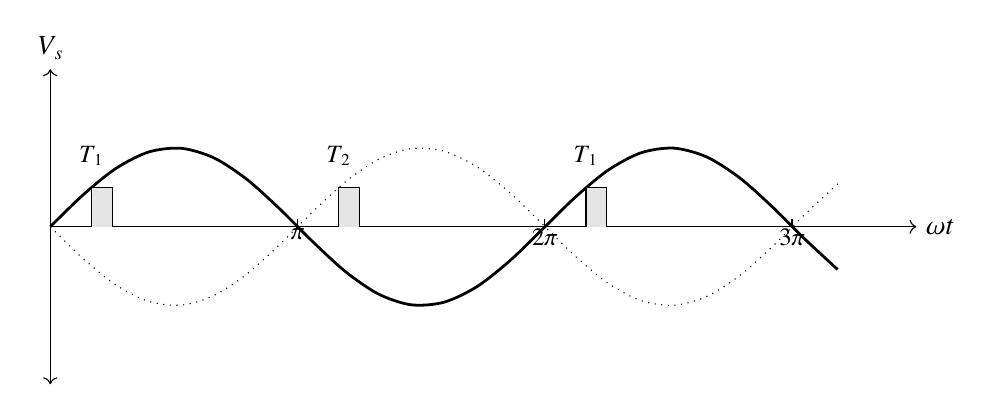
\begin{tikzpicture}[scale=1]
    \draw[->] (0,0) -- (11,0) node[right] {$\omega t$};
    \draw[<->] (0,-2) -- (0,2) node[above] {$V_s$};
    \draw[domain=0:10, smooth, variable=\x, black,line width=1pt] plot ({\x},{sin(deg(\x))});
    \draw[dotted,domain=0:10, smooth, variable=\x, black] plot ({\x},{-sin(deg(\x))});
    \foreach \x/\xtext in {3.14/\pi,6.28/2\pi,9.42/3\pi} {
        \draw (\x cm,0) -- (\x cm,0.1) node[below] {\small$\xtext$};
    }

\fill[gray!20] (0.5233,0) -- (0.5233,0.5) -- (0.785,0.5) -- (0.785,0) -- cycle;
    \fill[gray!20] (3.6633,0) -- (3.6633,0.5) -- (3.925,0.5) -- (3.925,0) -- cycle;
    \fill[gray!20] (6.8033,0) -- (6.8033,0.5) -- (7.065,0.5) -- (7.065,0) -- cycle;

    \draw (0.5233,0) -- (0.5233,0.5);
    \draw (0.5233,0.5) -- (0.785,0.5);
    \draw (0.785,0.5) -- (0.785,0);

    \draw (3.6633,0) -- (3.6633,0.5);
    \draw (3.6633,0.5) -- (3.925,0.5);
    \draw (3.925,0.5) -- (3.925,0);

    \draw (6.8033,0) -- (6.8033,0.5);
    \draw (6.8033,0.5) -- (7.065,0.5);
    \draw (7.065,0.5) -- (7.065,0);


     \node at (0.5233,0.9) {\small$T_1$};
     \node at (3.6633,0.9) {\small$T_2$};
     \node at (6.8033,0.9) {\small$T_1$};
\end{tikzpicture}
\end{figure}
\begin{figure}[!h]
    \centering
    \begin{tikzpicture}[scale=1]
    \draw[->] (0,0) -- (11,0) node[right] {$\omega t$};
    \draw[<->] (0,-2) -- (0,2) node[above] {$V_o$};
    \draw[domain=0.5233:3.14, smooth, variable=\x, black,line width=1pt] plot ({\x},{sin(deg(\x))});
    \draw[domain=3.6633:6.28, smooth, variable=\x, black,line width=1pt] plot ({\x},{-sin(deg(\x))});
    \draw[domain=6.8033:9.42, smooth, variable=\x, black,line width=1pt] plot ({\x},{sin(deg(\x))});

    \foreach \x/\xtext in {0.5233/\alpha, 3.14/\pi,4/\pi + \alpha ,6.28/2\pi,7.2/2\pi + \alpha,9.42/3\pi}{
        \draw (\x cm,0) -- (\x cm,0) node[below] {\small $\xtext$};
    }

     \draw [line width=1pt](0,0)--(0.5233,0);
    \draw [line width=1pt](0.5233,0) -- (0.5233,0.5);
    \draw[line width=1pt](3.14,0)-- (3.6633,0);
    \draw[line width=1pt] (3.6633,0) -- (3.6633,0.5);
    \draw [line width=1pt](6.28,0)--(6.8033,0);
    \draw [line width=1pt](6.8033,0) -- (6.8033,0.5);

    \node at (0.25,0.6){\small$T_2$};
    \node at (0.25,0.2){\small$D_2$};
     \node at (3.4,0.6){\small$T_1$};
    \node at (3.4,0.2){\small$D_1$};
    \node at (6.4,0.6){\small$T_2$};
    \node at (6.4,0.2){\small$D_2$};

    \node at (1.57,0.4){\small $T_1D_2$};
    \node at (4.71,0.4){\small $T_2D_1$};
    
\end{tikzpicture}
\end{figure}
\begin{figure}[!h]
    \centering
    \begin{tikzpicture}[scale=1]
    \draw[->] (0,0) -- (11,0) node[right] {$\omega t$};
    \draw[<->] (0,-2) -- (0,2) node[above] {$i_{T_1}$};
   
    \foreach \x/\xtext in {0.5233/\alpha,4/\pi + \alpha,7.2/2\pi + \alpha,10/3\pi + \alpha}{
        \draw (\x cm,0) -- (\x cm,0) node[below] {\small $\xtext$};
    }
     \draw [line width=1pt](0,0)--(0.5233,0);
    \draw [line width=1pt](0.5233,0) -- (0.5233,1);
    \draw[line width=1pt](0.5233,1)-- (3.6633,1);
    \draw[line width=1pt] (3.6633,1) -- (3.6633,0);
    \draw[line width=1pt] (3.6633,0) -- (6.8033,0);
    \draw [line width=1pt](6.8033,0)--(6.8033,1);
    \draw [line width=1pt](6.8033,1) -- (9.948,1);
     \draw [line width=1pt] (9.948,1) -- (9.948,0);

     \draw[dotted,domain=0:10, smooth, variable=\x, black] plot ({\x},{1});
     \node at (0.4,1.2) {\small $I_{DC}$};
\end{tikzpicture}
\end{figure}
\begin{figure}[!h]
    \centering
    \begin{tikzpicture}[scale=1]
    \draw[->] (0,0) -- (11,0) node[right] {$\omega t$};
    \draw[<->] (0,-2) -- (0,2) node[above] {$i_{s}$};
   

    \draw [line width=1pt](0.5233,0) -- (0.5233,1);
    \draw[line width=1pt](0.5233,1)-- (3.14,1);
    \draw[line width=1pt](3.14,1)-- (3.14,0);
    \draw[line width=1pt] (3.14,0) -- (3.6633,0);
    \draw[line width=1pt] (3.6633,0) -- (3.6633,-1);
    \draw[line width=1pt] (3.6633,-1) -- (6.28,-1);
    \draw[line width=1pt]  (6.28,-1) -- (6.28,0);
    \draw[line width=1pt] (6.28,0) -- (6.8033,0);
    \draw [line width=1pt](6.8033,0)--(6.8033,1);
    \draw [line width=1pt](6.8033,1) -- (9.42,1);
     \draw [line width=1pt] (9.42,1) -- (9.42,0);
     \draw [line width=1pt] (9.42,0) -- (9.948,0);

     \draw[dotted,domain=0:10, smooth, variable=\x, black] plot ({\x},{1});
     \node at (0.4,1.2) {\small $I_{DC}$};
    
\end{tikzpicture}
\end{figure}

From \tabref{tab:inputs.EE.59.2022}:
\begin{align}
   (I_{s_1})_{peak} &= \frac{4I_{dc}}{\pi}\cos{\left(\frac{\alpha}{2}\right)}\\
    &= \frac{4 \times 15 }{\pi}\times \cos{\frac{45 \degree}{2}}\\
    &=17.64 A 
\end{align}

%\end{document}

\newpage
 \item The output of the system y\brak{t} is related to its input x\brak{t} according to the relation $y\brak{t}=x\brak{t}sin\brak{2\pi t}$.This system is 
\\\\\brak{A} Linear and time-variant
\\\brak{B} Non-Linear and time-invariant
\\\brak{C} Linear and time-invariant
\\\brak{D} Non-linear and time-variant
\\\hfill(GATE 2022 IN Question 14)
\solution
\iffalse
\let\negmedspace\undefined
\let\negthickspace\undefined
\documentclass[journal,12pt,twocolumn]{IEEEtran}
\usepackage{cite}
\usepackage{amsmath,amssymb,amsfonts,amsthm}
\usepackage{algorithmic}
\usepackage{graphicx}
\usepackage{textcomp}
\usepackage{xcolor}
\usepackage{txfonts}
\usepackage{listings}
\usepackage{enumitem}
\usepackage{mathtools}
\usepackage{gensymb}
\usepackage{comment}
\usepackage[breaklinks=true]{hyperref}
\usepackage{tkz-euclide} 
\usepackage{listings}
\usepackage{gvv}                                        
\def\inputGnumericTable{}                                 
\usepackage[latin1]{inputenc}                                
\usepackage{color}                                            
\usepackage{array}                                            
\usepackage{longtable}                                       
\usepackage{calc}                                             
\usepackage{multirow}                                         
\usepackage{hhline}                                           
\usepackage{ifthen}                                           
\usepackage{lscape}

\newtheorem{theorem}{Theorem}[section]
\newtheorem{problem}{Problem}
\newtheorem{proposition}{Proposition}[section]
\newtheorem{lemma}{Lemma}[section]
\newtheorem{corollary}[theorem]{Corollary}
\newtheorem{example}{Example}[section]
\newtheorem{definition}[problem]{Definition}
\newcommand{\BEQA}{\begin{eqnarray}}
\newcommand{\EEQA}{\end{eqnarray}}
\newcommand{\define}{\stackrel{\triangle}{=}}
\theoremstyle{remark}
\newtheorem{rem}{Remark}
\begin{document}

\bibliographystyle{IEEEtran}
\vspace{3cm}

\title{GATE 2022 IN 14}
\author{EE23BTECH11065 - prem sagar}
\maketitle
\newpage

\bigskip

\renewcommand{\thefigure}{\theenumi}
\renewcommand{\thetable}{\theenumi}
\textbf{Question}:
\\The output of the system y\brak{t} is related to its input x\brak{t} according to the relation $y\brak{t}=x\brak{t}sin\brak{2\pi t}$.This system is 
\\\\\brak{A} Linear and time-variant
\\\brak{B} Non-Linear and time-invariant
\\\brak{C} Linear and time-invariant
\\\brak{D} Non-linear and time-variant
\\\textbf{Solution}:
\fi
\begin{table}[!ht]
\def\arraystretch{1.5}
   \centering
    \renewcommand\thetable{1}
      \begin{tabular}{|c|c|c|}
   \hline
   \textbf{Symbol} & \textbf{Value}& \textbf{Description} \\
   \hline
         $x\brak{t}$ & & input signal\\
        \hline
        $y\brak{t}$ &$x\brak{t}sin\brak{2\pi t}$  & output signal\\
        \hline
        $\tau$ &   & Time delay\\
        \hline
\end{tabular}

    \caption{input parameters}
    \label{tab:IN 14}
 \end{table}
\\ From \tabref{tab:IN 14}
\\\begin{align}
y_1\brak{t}&\leftrightarrow x_1\brak{t}
\\y_2\brak{t}&\leftrightarrow x_2\brak{t}
\\ay_1\brak{t}+by_2\brak{t}&\leftrightarrow ax_1\brak{t}+bx_2\brak{t}
\\ay_1\brak{t}+by_2\brak{t}&=\brak{ax_1\brak{t}+bx_2\brak{t}}sin\brak{2\pi t}
\end{align}
\\$\therefore$ satisfies principle of superposition
\begin{align}
ky\brak{t}&\leftrightarrow kx\brak{t}
\\ky\brak{t}&=k\brak{x\brak{t}sin\brak{2\pi t}}
\end{align}
\\$\therefore$ satisfies principle of homogenity
\\$\therefore$ it is linear
\\\\Delay in input x\brak{t}:
\begin{align}
y_1\brak{t}&=x\brak{t-\tau}sin\brak{2\pi t}
\end{align}
\\\\Delay in output y\brak{t}:
\begin{align}
y\brak{t-\tau}&=x\brak{t-\tau}sin\brak{2\pi\brak{t-\tau}}
\\y_2\brak{t}&=x\brak{t-\tau}sin\brak{2\pi\brak{t-\tau}}
\\y_1\brak{t}&\neq y_2\brak{t}
\end{align}
\\$\therefore$ it is time variant
\\$\therefore$ \brak{A} linear and time variant

\newpage
\item Two linear time-invariant systems with transfer functions 
    \begin{align*}
    G_{1}\brak{s} = \frac{10}{s^{2} + s + 1} 
    \end{align*}
    and
    \begin{align*}
    G_{2}\brak{s} = \frac{10}{s^{2}+s\sqrt{10} +10}
    \end{align*}
    have unit step responses $y_{1}\brak{t}$ and $y_{2}\brak{t}$, respectively. Which of the following statements is/are true?
    \begin{enumerate}
    \item $y_{1}\brak{t}$ and $y_{2}\brak{t}$ have the same percentage peak overshoot.\\
    \item $y_{1}\brak{t}$ and $y_{2}\brak{t}$ have the same steady state values.\\
    \item $y_{1}\brak{t}$ and $y_{2}\brak{t}$ have the same damped frequency of oscillation.\\
    \item $y_{1}\brak{t}$ and $y_{2}\brak{t}$ have the same $2\%$ settling time.\\
    \end{enumerate}
    \hfill(GATE 2022 EC Q50)\\
    \solution
    \iffalse
\documentclass[journal,12pt,onecolumn]{IEEEtran}
\usepackage{cite}
\usepackage{amsmath,amssymb,amsfonts,amsthm}
\usepackage{algorithmic}
\usepackage{graphicx}
\usepackage{textcomp}
\usepackage{xcolor}
\usepackage{txfonts}
\usepackage{listings}
\usepackage{enumitem}
\usepackage{mathtools}
\usepackage{gensymb}
\usepackage{comment}
\usepackage[breaklinks=true]{hyperref}
\usepackage{tkz-euclide}
\usepackage{listings}
\usepackage{gvv}
\def\inputGnumericTable{}
\usepackage[latin1]{inputenc}
\usepackage{color}
\usepackage{array}
\usepackage{longtable}
\usepackage{calc}
\usepackage{multirow}
\usepackage{hhline}
\usepackage{ifthen}
\usepackage{lscape}

\newtheorem{theorem}{Theorem}[section]
\newtheorem{problem}{Problem}
\newtheorem{proposition}{Proposition}[section]
\newtheorem{lemma}{Lemma}[section]
\newtheorem{corollary}[theorem]{Corollary}
\newtheorem{example}{Example}[section]
\newtheorem{definition}[problem]{Definition}
\newcommand{\BEQA}{\begin{eqnarray}}
    \newcommand{\EEQA}{\end{eqnarray}}
\newcommand{\define}{\stackrel{\triangle}{=}}
\theoremstyle{remark}
\newtheorem{rem}{Remark}

\begin{document}
    
    \bibliographystyle{IEEEtran}
    \vspace{3cm}
    
    \title{Gate 2022 EC Q50}
    \author{EE23BTECH11212 - Manugunta Meghana Sai$^{*}$% <-this % stops a space
    }
    \maketitle
    \bigskip
    
    \renewcommand{\thefigure}{\theenumi}
    \renewcommand{\thetable}{\theenumi}
    
    \vspace{3cm}
    \textbf{Gate 2022 EC Q50} 
    
    Two linear time-invariant systems with transfer functions 
    \begin{align*}
    G_{1}\brak{s} = \frac{10}{s^{2} + s + 1} 
    \end{align*}
    and
    \begin{align*}
    G_{2}\brak{s} = \frac{10}{s^{2}+s\sqrt{10} +10}
    \end{align*}
    have unit step responses $y_{1}\brak{t}$ and $y_{2}\brak{t}$, respectively. Which of the following statements is/are true?
    \begin{enumerate}
    \item $y_{1}\brak{t}$ and $y_{2}\brak{t}$ have the same percentage peak overshoot.\\
    \item $y_{1}\brak{t}$ and $y_{2}\brak{t}$ have the same steady state values.\\
    \item $y_{1}\brak{t}$ and $y_{2}\brak{t}$ have the same damped frequency of oscillation.\\
    \item $y_{1}\brak{t}$ and $y_{2}\brak{t}$ have the same $2\%$ settling time.\\
    \end{enumerate}
    \solution
    \fi
    \begin{table}[h!]
 	\centering
 	\resizebox{6 cm}{!}{
 		\begin{tabular}{|c|c|c|}
	\hline
	\textbf{Parameter} &  \textbf{Description} & \textbf{value}\\[6pt]
	\hline
	$X_{1}\brak{s}$ & input & $\frac{1}{s}$ \\[6pt]
	\hline
	$X_{2}\brak{s}$ & input & $\frac{1}{s}$ \\[6pt]
	\hline
	$G_{1}\brak{s}$ & transfer function & $\frac{10}{s^{2} + s + 1} $ \\[6pt]
	\hline
	$G_{2}\brak{s}$ & transfer function & $\frac{10}{s^{2}+s\sqrt{10} +10} $ \\[6pt]
	\hline
	$y_{1}\brak{t}$ & unit step response & $-$\\[6pt]
	\hline
	$y_{2}\brak{t}$ & unit step response & $-$\\[6pt]
	\hline
	$\omega_{n}$ & natural frequency & $-$\\[6pt]
	\hline
	$\zeta$ & damping ratio & $-$\\[6pt]
	\hline 
	
\end{tabular}

 	}
 	\caption{Given Parameters}
 	\label{tab:msmECgate50tab1}
     \end{table} 
    The general second-order transfer function is given by:
    \begin{align}
    G\brak{s} = \frac{\omega_n^2}{s^2 + 2\zeta\omega_n s + \omega_n^2}
    \end{align}
    After comparing the coefficients of $G_{1}\brak{s}$ and $G_{2}\brak{s}$,
    \begin{table}[h!]
 	\centering
 	\resizebox{6 cm}{!}{
 		\begin{tabular}{|c|c|c|}
	\hline
	\textbf{Tranfer function} &  $\omega_{n}$ & $\zeta$\\[6pt]
	\hline
	$G_{1}\brak{s}$ & $1$ & $\frac{1}{2}$ \\[6pt]
	\hline
	$G_{1}\brak{s}$ & $\sqrt{10}$ & $\frac{1}{2}$ \\[6pt]
	\hline
\end{tabular}

 	}
 	\caption{Given Parameters}
 	\label{tab:msmECgate50tab2}
     \end{table} 
    as $\zeta = \frac{1}{2}$ is less than 1, the system is underdamped.
    \begin{align}
    Y\brak{s} &= X\brak{s} G\brak{s}\\
    &= \frac{1}{s} \brak{\frac{\omega_n^2}{s^2 + 2\zeta\omega_n s + \omega_n^2}}  
    \end{align}
    Applying inverse laplace transform,
    \begin{equation}
    y(t) = 1 - \frac{e^{-\zeta \omega_n t}}{1 - \zeta^2} \sin(\omega_d t + \phi)
    \label{eq:EC50msm}
    \end{equation}
    where $\omega_{d}$ is the damped frequency of oscillation.
    \begin{equation}
    \omega_{d} = \omega_{n}\sqrt{1 - {\zeta}^2}
    \label{eq:EC50msm2eq}
    \end{equation}
    The percentage peak overshoot $\brak{PO}$:
    \begin{equation}
    PO = \left( \frac{y_{\text{max}} - y_{\text{ss}}}{y_{\text{ss}}} \right) \times 100\%
    \label{eq:EC50msm1eq}
    \end{equation}
    $y_{\text{max}}$ is obtained by differentiating~\eqref{eq:EC50msm} with respect to time and equating it to zero, substituting the value in~\eqref{eq:EC50msm},
    \begin{align}
    y_{\text{max}} = 1 + \frac{1}{\sqrt{1-{\zeta}^2}}
    \end{align}
    $y_{\text{ss}}$ is obtained by final value theorem,
    \begin{align}
    y_{\text{ss}} &= \lim_{{s \to 0}} sY(s)\\
    &= \lim_{{s \to 0}} s\frac{\omega_n^2}{s^2 + 2\zeta\omega_n s + \omega_n^2} \frac{1}{s}\\
    &= 1
    \end{align} 
    Substituting the values of $y_{\text{max}}$ and $y_{\text{ss}}$ in~\eqref{eq:EC50msm1eq}, 
    \begin{align}
    PO = \frac{1}{\sqrt{1-{\zeta}^2}} \times 100\%
    \end{align}
    $y_{1}\brak{t}$ and $y_{2}\brak{t}$ have same $\zeta$, they have same percentage peak overshoot.So, option $\brak{1}$ is correct.\\
    The steady state value of $y\brak{t}$ is given by final value theorem:
    \begin{align}
    y_{1ss} &= \lim_{{s \to 0}} sY_{1}(s)\\
    &= \lim_{{s \to 0}} s \frac{10}{s^{2} + s + 1}  \frac{1}{s}\\
    &= 10\\
    y_{2ss} &= \lim_{{s \to 0}} sY_{2}(s)\\
    &= \lim_{{s \to 0}} s \frac{10}{s^{2}+s\sqrt{10} +10}  \frac{1}{s}\\
    &= 1
    \end{align} 
    as both the unit step responses have different steady state values, option $\brak{2}$ is incorrect.\\
    From~\eqref{eq:EC50msm1eq}, as $\omega_{n}$ is different for $y_{1}\brak{t}$ and $y_{2}\brak{t}$, they have different damped frequency of oscillation. Hence option $\brak{3}$ is incorrect.\\
    Settling time $T_s$:
    \begin{align}
    T_s = \frac{4}{\zeta \omega_n}
    \end{align}
    As, $\omega_{n}$ is different for $y_{1}\brak{t}$ and $y_{2}\brak{t}$, they have different $2\%$ settling time, Hence option $\brak{4}$ is incorrect.\\
    So, only option $\brak{1}$ is correct.   
%\end{document}

    \newpage
\item Consider a single-input-single-output (SISO) system with the transfer function
\begin{align*}
G_p(s) = \frac{2\brak{s+1}}{\brak{\frac{1}{2}s+1}\brak{\frac{1}{4}s+1}}
\end{align*}
where the time constants are in minutes. The system is forced by a unit step input at
time $t = 0$. The time at which the output response reaches the maximum is \rule{1cm}{0.15mm} minutes (rounded off to two decimal places). \hfill (GATE CH 2022)\\
\solution
\input{2022/CH/60/60.tex}
\newpage
\item Consider the system as shown below:
\begin{center}
\begin{tikzpicture}
    % Box
    \draw (0,0) rectangle (4,2);

    % Arrow and label for x(t)
    \draw[->,>=stealth] (-1,1) -- node[above] {$x(t)$} (0,1);

    % Arrow and label for y(t)
    \draw[->,>=stealth] (4,1) -- node[above] {$y(t)$} (5,1);
\end{tikzpicture}
\end{center}


The system is described by the equation
\[ y(t) = x(e^{-t}). \]\\
The system is:
\begin{itemize}
    \item[(A)] non-linear and causal.
    \item[(B)] linear and non-causal.
    \item[(C)] non-linear and non-causal.
    \item[(D)] linear and causal.
\end{itemize}
\hfill(GATE EE 2022)\\
 \iffalse
\documentclass{article}
\usepackage{tikz}
\usepackage{amsmath}

\begin{document}
Consider the system as shown below:
\let\negmedspace\undefined
\let\negthickspace\undefined
\documentclass[journal,12pt,twocolumn]{IEEEtran}
\usepackage{cite}
\usepackage{amsmath,amssymb,amsfonts,amsthm}
\usepackage{algorithmic}
\usepackage{graphicx}
\usepackage{textcomp}
\usepackage{xcolor}
\usepackage{txfonts}
\usepackage{listings}
\usepackage{enumitem}
\usepackage{mathtools}
\usepackage{gensymb}
\usepackage{comment}
\usepackage[breaklinks=true]{hyperref}
\usepackage{tkz-euclide} % loads  TikZ and tkz-base
\usepackage{listings}
\usepackage[latin1]{inputenc}                                
\usepackage{color}                                            
\usepackage{array}                                            
\usepackage{longtable}                                       
\usepackage{calc}                                             
\usepackage{multirow}                                         
\usepackage{hhline}                                           
\usepackage{ifthen}                                           
\usepackage{lscape}
\usepackage{caption}
\usepackage{subcaption}
\usepackage{float}
\usepackage{circuitikz}
\usetikzlibrary{decorations.markings} 


\newtheorem{theorem}{Theorem}[section]
\newtheorem{problem}{Problem}
\newtheorem{proposition}{Proposition}[section]
\newtheorem{lemma}{Lemma}[section]
\newtheorem{corollary}[theorem]{Corollary}
\newtheorem{example}{Example}[section]
\newtheorem{definition}[problem]{Definition}
%\newtheorem{thm}{Theorem}[section] 
%\newtheorem{defn}[thm]{Definition}
%\newtheorem{algorithm}{Algorithm}[section]
%\newtheorem{cor}{Corollary}
\newcommand{\BEQA}{\begin{eqnarray}}
\newcommand{\EEQA}{\end{eqnarray}}
\newcommand{\define}{\stackrel{\triangle}{=}}
\theoremstyle{remark}
\newtheorem{rem}{Remark}
%\bibliographystyle{ieeetr}

\begin{document}

%
\providecommand{\pr}[1]{\ensuremath{\Pr\left(#1\right)}}
\providecommand{\prt}[2]{\ensuremath{p_{#1}^{\left(#2\right)} }}        % own macro for this question
\providecommand{\qfunc}[1]{\ensuremath{Q\left(#1\right)}}
\providecommand{\sbrak}[1]{\ensuremath{{}\left[#1\right]}}
\providecommand{\lsbrak}[1]{\ensuremath{{}\left[#1\right.}}
\providecommand{\rsbrak}[1]{\ensuremath{{}\left.#1\right]}}
\providecommand{\brak}[1]{\ensuremath{\left(#1\right)}}
\providecommand{\lbrak}[1]{\ensuremath{\left(#1\right.}}
\providecommand{\rbrak}[1]{\ensuremath{\left.#1\right)}}
\providecommand{\cbrak}[1]{\ensuremath{\left\{#1\right\}}}
\providecommand{\lcbrak}[1]{\ensuremath{\left\{#1\right.}}
\providecommand{\rcbrak}[1]{\ensuremath{\left.#1\right\}}}
\newcommand{\sgn}{\mathop{\mathrm{sgn}}}
\providecommand{\abs}[1]{\left\vert#1\right\vert}
\providecommand{\res}[1]{\Res\displaylimits_{#1}} 
\providecommand{\norm}[1]{\left\lVert#1\right\rVert}
%\providecommand{\norm}[1]{\lVert#1\rVert}
\providecommand{\mtx}[1]{\mathbf{#1}}
\providecommand{\mean}[1]{E\left[ #1 \right]}
\providecommand{\cond}[2]{#1\middle|#2}
\providecommand{\fourier}{\overset{\mathcal{F}}{ \rightleftharpoons}}
\newenvironment{amatrix}[1]{%
  \left(\begin{array}{@{}*{#1}{c}|c@{}}
}{%
  \end{array}\right)
}
%\providecommand{\hilbert}{\overset{\mathcal{H}}{ \rightleftharpoons}}
%\providecommand{\system}{\overset{\mathcal{H}}{ \longleftrightarrow}}
        %\newcommand{\solution}[2]{\textbf{Solution:}{#1}}
\newcommand{\solution}{\noindent \textbf{Solution: }}
\newcommand{\cosec}{\,\text{cosec}\,}
\providecommand{\dec}[2]{\ensuremath{\overset{#1}{\underset{#2}{\gtrless}}}}
\newcommand{\myvec}[1]{\ensuremath{\begin{pmatrix}#1\end{pmatrix}}}
\newcommand{\mydet}[1]{\ensuremath{\begin{vmatrix}#1\end{vmatrix}}}
\newcommand{\myaugvec}[2]{\ensuremath{\begin{amatrix}{#1}#2\end{amatrix}}}
\providecommand{\rank}{\text{rank}}
\providecommand{\pr}[1]{\ensuremath{\Pr\left(#1\right)}}
\providecommand{\qfunc}[1]{\ensuremath{Q\left(#1\right)}}
        \newcommand*{\permcomb}[4][0mu]{{{}^{#3}\mkern#1#2_{#4}}}
\newcommand*{\perm}[1][-3mu]{\permcomb[#1]{P}}
\newcommand*{\comb}[1][-1mu]{\permcomb[#1]{C}}
\providecommand{\qfunc}[1]{\ensuremath{Q\left(#1\right)}}
\providecommand{\gauss}[2]{\mathcal{N}\ensuremath{\left(#1,#2\right)}}
\providecommand{\diff}[2]{\ensuremath{\frac{d{#1}}{d{#2}}}}
\providecommand{\myceil}[1]{\left \lceil #1 \right \rceil }
\newcommand\figref{Fig.~\ref}
\newcommand\tabref{Table~\ref}
\newcommand{\sinc}{\,\text{sinc}\,}
\newcommand{\rect}{\,\text{rect}\,}
%%
%       %\newcommand{\solution}[2]{\textbf{Solution:}{#1}}
%\newcommand{\solution}{\noindent \textbf{Solution: }}
%\newcommand{\cosec}{\,\text{cosec}\,}
%\numberwithin{equation}{section}
%\numberwithin{equation}{subsection}
%\numberwithin{problem}{section}
%\numberwithin{definition}{section}
%\makeatletter
%\@addtoreset{figure}{problem}
%\makeatother

%\let\StandardTheFigure\thefigure
\let\vec\mathbf

\bibliographystyle{IEEEtran}

\vspace{3cm}
\title{Assignment}
\author{EE23BTECH11001 - Aashna Sahu}
\maketitle
\bigskip

\renewcommand{\thefigure}{\theenumi}
\renewcommand{\thetable}{\theenumi}
%\renewcommand{\theequation}{\theenumi}

Q:An ideal OPAMP circuit with a sinusoidal input is shown in the figure. The 3dB frequency is the frequency at which the magnitude of the voltage gain decreases by 3 dB from the maximum value. Which of the options is/are correct?

\begin{figure}[H]
  \centering
  \begin{circuitikz}

\ctikzset{bipoles/length=1cm}                           
\draw (0, 0) node[op amp] (opamp) {};
\draw (opamp.-) to[R,l_= $1k\Omega$,-] (-2.5, 0.35) -- (-2.7, 0.35) to[C,l_=$1\mu F$,-](-3.35,0.35)  (-3.25,-0.5) node[ground]{};                                 
\draw (opamp.-) to[short,*-] ++(0,0.5) coordinate (leftC) to[R= $2k\Omega$] (leftC -| opamp.out)to[short,-*] (opamp.out) to [short,-*] (1.5,0) (1.5,-0.5) node[ground]{};
\draw (opamp.+) -- (-1,-0.35) to (-1,-0.5) node[ground]{}
;
\draw[thick] (opamp.up) -- +(0,0.2) node[right] {\scriptsize$+15V$};
\draw[thick] (opamp.down) -- +(0,-0.2) node[right] {\scriptsize$-15V$};

% Double-sided arrows for input and output voltage
%\draw[thick,postaction={decorate,decoration={markings,mark=at position 1.0 with {\arrow{stealth}}}}] (-3.35,-0.5) -- (-3.35,0.30) node[midway,left] {$V_{in}$};
%\draw[postaction={decorate,decoration={markings,mark=at position 1.0 with {\arrow{stealth}}}}] (-3.35,0.30) -- (-3.35,-0.5){};
%\draw[thick,postaction={decorate,decoration={markings,mark=at position 1.0 with {\arrow{stealth}}}}] (1.6,0) -- (1.6,-0.7) node[midway,right] {$V_{out}$};
%\draw[postaction={decorate,decoration={markings,mark=at position 1.0 with {\arrow{stealth}}}}] (1.6,-0.7) -- (1.6,0) {};
 
 
\draw[thick, postaction={decorate,decoration={markings,mark=at position 0 with {\node[left] {\scriptsize$-$}; \draw[-latex](0.2,0)--(0,0);},mark=at position 1 with {\node[left] {\scriptsize$+$}; \draw[-latex] (0,0)--(0.2,0);}}}] (-3.35,-0.7) -- (-3.35,0.1) node[midway,left] {\scriptsize$V_{in}$};
\draw[thick, postaction={decorate,decoration={markings,mark=at position 0 with {\node[right] {\scriptsize$+$}; \draw[-latex] (0.2,0)--(0,0);},mark=at position 1 with {\node[right] {\scriptsize$-$}; \draw[-latex] (0,0)--(0.3,0);}}}] (1.6,0) -- (1.6,-0.5) node[midway,right] {\scriptsize$V_{out}$};
                                                          \end{circuitikz}                                        


  \label{fig:fig1}
\end{figure}



\begin{enumerate}[label=(\Alph*)]
\item The circuit is a low pass filter.\\
\item The circuit is a high pass filter.\\
\item The 3 dB frequency is 1000rad/s.\\
\item The 3 dB frequency is $\frac{1000}{3}$rad/s.\\
\end{enumerate}
\hfill(GATE EC 2022)

\solution

\begin{table}[ht]
  \centering
  \begin{table}[!ht] 
\centering
\setlength{\extrarowheight}{8pt}
\begin{tabular}{|l|l|l|}
    \hline
    \textbf{Parameter} & \textbf{Description} & \textbf{Values}\\
    \hline
     m & load of system &  \\
    \hline
     k & stiffness of system &  \\
    \hline
     $\omega_n$ & Natural frequency & $\sqrt{\frac{k}{m}}$ \\
    \hline
    $\zeta$ & Damping ratio & $\frac{c}{2m\omega_n}$ \\
    \hline
     y\brak{t} & Output of system & \\
    \hline
     x\brak{t} & Input to the system & \\
    \hline
     c & Damping coefficient & \\
    \hline
    T\brak{s} & Transfer function of system & $\frac{Y\brak{s}}{R\brak{s}}$\\
    \hline
  \end{tabular}
  \vspace{4mm}
 \caption{Parameter Table}
 \label{tab:table0_ee_22_39}
\end{table}

  \caption{Input Parameters}
  \label{tab:tab1}
\end{table}

\begin{figure}[H]
  \centering
  \input{codes/circuit2.tex}
  \label{fig:fig1}
\end{figure}

\begin{align}
\frac{V_{in}-V}{\frac{1}{sC}+R_1}=\frac{V-V_{out}}{R_2}
\end{align}
As Op-Amp is ideal
\begin{align}
V=V^+=0V\\
\abs{\frac{V_{out}}{V_{in}}}=\frac{sCR_2}{1+sCR_1}\\
H(s)=\frac{sCR_2}{1+sCR_1}
\label{eq:eq4}
\end{align}
Keeping $s=j\omega$\\
For determining nature of Filter\\
Put $j\omega=0$
\begin{align}
H(j\omega)=0
\end{align}
Put $j\omega\rightarrow \infty$
\begin{align}
H(j\omega)=\frac{R_2}{R_1}=2\quad (\text{Finite})
\end{align}\\
$\therefore$ It is high pass filter.\\

On simplifying \eqref{eq:eq4} further
\begin{align}
H(j\omega)=\frac{R_2}{R_1}\left(\frac{j\omega}{j\omega+\frac{1}{CR_1}}\right)\\
\abs{H(j\omega)}_{max}=\frac{R_2}{R_1} \label{eq:eq8}\\
\abs{H(j\omega)}_{\omega=\omega_c}=\frac{R_2}{R_1}\abs{\frac{j\omega_c}{j\omega_c+\frac{1}{CR_1}}}
\label{eq:eq9}
\end{align}
%\textbf{Alternate}\\
%Generally for first order transfer function

%\begin{align}
%H(s)|_{LPF}=\frac{1}{s+\omega}\\
%H(s)|_{HPF}=\frac{s}{s+\omega}
%\label{eq:eq8}
%\end{align}
Given: 
\begin{align}
20\log(\abs{H(j\omega)}_{max})-20\log(\abs{H(j\omega)}_{\omega=\omega_c})=3 dB
\end{align}
\begin{align}
\frac{\abs{H(j\omega)}_{max}}{\abs{H(j\omega)}_{\omega=\omega_c}}=\sqrt 2
\end{align}
 
From \eqref{eq:eq8} and \eqref{eq:eq9}
\begin{align}
\frac{R_2}{R_1}\abs{\frac{j\omega_c}{j\omega_c+\frac{1}{CR_1}}}&=\frac{1}{\sqrt 2}\frac{R_2}{R_1}\\
\abs{\frac{j\omega_c}{j\omega_c+\frac{1}{CR_1}}}&=\frac{1}{\sqrt 2}\\
\implies \omega_c &= \frac{1}{CR_1}
\end{align}
From \tabref{tab:tab1}
\begin{align}
\omega_c= 1000 \text{rad/s}
\end{align}
Where $\omega_c$ is 3 dB frequency.\\

Finally, Correct options are (B) and (C).

\begin{figure}[H]
  \centering
  \includegraphics[width=1.0\columnwidth]{figs/plot1.png}
  \caption{\centering Frequency response plot}
  \label{fig:fig1}
\end{figure}
\end{document}




The system is described by the equation
\[ y(t) = x(e^{-t}). \]

The system is:
\begin{itemize}
    \item[(A)] non-linear and causal.
    \item[(B)] linear and non-causal.
    \item[(C)] non-linear and non-causal.
    \item[(D)] linear and causal.
\end{itemize}
\fi
\textbf{Solution:}\\

\textbf{Homogeneity Test:}\\
For input \(x_1(e^{-t})\), the output will be \(y_1(t)\).
\begin{align}
y_1(t) = x_1(e^{-t})
\end{align}
Multiplying both sides by a scalar quantity 'a'
\begin{align}
ay_1(t) = ax_1(e^{-t})
\end{align}
For input \(x_2(e^{-t})\), the output will be \(y_2(t)\).
\begin{align}
y_2(t) = x_2(e^{-t})
\end{align}
Multiplying both sides by a scalar quantity 'b'
\begin{align}
by_2(t) = bx_2(e^{-t})
\end{align}
Adding the above equations we get:
\begin{align}
ay_1(t) + by_2(t) = ax_1(e^{-t}) + bx_2(e^{-t})
\end{align}
Let us assume that, for input \(ax_1(e^{-t}) + bx_2(e^{-t})\), the output will be \(y_3(t)\).
\begin{align}
y_3(t) = ax_1(e^{-t}) + bx_2(e^{-t})
\end{align}
But, \(ay_1(t) + by_2(t) = ax_1(e^{-t}) + bx_2(e^{-t})\)\\
Therefore;
\begin{align}
y_3(t) = ay_1(t) + by_2(t)
\end{align}

The system satisfies homogeneity, as scaling the input scales the output.\\

\textbf{Additivity Test:}\\
From the given system;
\begin{align}
y(t) = x(e^{-t})
\end{align}
\begin{align}
y(0) = x(e^{0})
\end{align}
\begin{align}
y(1) = x(e) = x(2.71)
\end{align}
So, the present value of output depends on the future value of input, indicating non-causality.

Therefore, the correct answer is:
\textbf{(B) linear and non-causal}

\end{document}


\newpage
\item The block diagrams of an ideal system and a real system with their impulse
responses are shown below. An auxiliary path is added to the delayed impulse
response in the real system.\\
\\
For a unit impulse input $\brak{x\brak{t}} = \delta \brak{t}$ to both systems, gain $\beta$ is chosen such that $y \brak{4T}$ is same for both systems. The value of $\beta$ is:
\begin{figure}[ht]
    \centering
    \includegraphics[width=\columnwidth]{2022/BM/40/figs/fig3.png}
    \label{fig: 10.5.3.128}
\end{figure}
\\
$\brak{A} e^{-3 \alpha T} \brak{1 - e^{-2 \alpha T}}$\\
\\
$\brak{B} -e^{- \alpha T} \brak{1 - e^{-3 \alpha T}}$\\
\\
$\brak{C} -e^{-3 \alpha T} \brak{1 - e^{-\alpha T}}$\\
\\
$\brak{D} e^{-2 \alpha T} \brak{1 - e^{-2 \alpha T}}$\\
\hfill(GATE BM 2022)\\
\solution
\input{2022/BM/40/GATE2022_BM_40.tex}
\newpage

\item  In a unity-gain feedback control system, the plant
$P(s) = \frac{0.001}{s\brak{2s+1}\brak{0.01s+1}}$
is controlled by a lag compensator
$C(s) = \frac{s+10}{s+0.1}$
The slope (in dB/decade) of the asymptotic Bode magnitude plot of the loop gain
at $\omega= 3 $rad/s is \_\_\_\_\_\_\_\_ (in integer)
\hfill(GATE 2022 IN)\\
\solution
 \iffalse
\let\negmedspace\undefined
\let\negthickspace\undefined
\documentclass[journal,12pt,onecolumn]{IEEEtran}
\usepackage{cite}
\usepackage{amsmath,amssymb,amsfonts,amsthm}
\usepackage{algorithmic}
\usepackage{graphicx}
\usepackage{textcomp}
\usepackage{xcolor}
\usepackage{txfonts}
\usepackage{listings}
\usepackage{enumitem}
\usepackage{mathtools}
\usepackage{gensymb}
\usepackage{comment}
\usepackage[breaklinks=true]{hyperref}
\usepackage{tkz-euclide} 
\usepackage{tikz}
\usepackage{circuitikz}
%\usetikzlibrary{circuits.ee.IEC}
\usepackage{listings}
\usepackage{gvv} 
\usepackage{caption}
\def\inputGnumericTable{}                   

%\usepackage[latin1]{inputenc}                                
\usepackage{color}                                            
\usepackage{array}                                            
\usepackage{longtable}                                       
\usepackage{calc}                                             
\usepackage{multirow}                                         
\usepackage{hhline}                                           
\usepackage{ifthen}                                           
\usepackage{lscape}
\usepackage{tikz}
\usepackage{circuitikz}

\newtheorem{theorem}{Theorem}[section]
\newtheorem{problem}{Problem}
\newtheorem{proposition}{Proposition}[section]
\newtheorem{lemma}{Lemma}[section]
\newtheorem{corollary}[theorem]{Corollary}
\newtheorem{example}{Example}[section]
\newtheorem{definition}[problem]{Definition}
\newcommand{\BEQA}{\begin{eqnarray}}
\newcommand{\EEQA}{\end{eqnarray}}
\newcommand{\define}{\stackrel{\triangle}{=}}
\theoremstyle{remark}
\newtheorem{rem}{Remark}

\begin{document}

\bibliographystyle{IEEEtran}
\vspace{3cm}

\title{GATE: EE - 59.2022}
\author{EE23BTECH11013 - Avyaaz$^{*}$% <-this % stops a space 
}
\maketitle
% \newpage
% \bigskip

\renewcommand{\thefigure}{\arabic{figure}}
\renewcommand{\thetable}{\arabic{table}}

\large\textbf{\textsl{Question:}}
For the ideal AC-DC rectifier circuit shown in the figure below, the load current
magnitude is $I_{dc}$ = $15$ A and is ripple free. The thyristors are fired with a delay angle
of 45\degree
. The amplitude of the fundamental component of the source current, in
amperes, is \_\_\_\_\_\_\_\_{\em (Round off to 2
decimal places)}. \hfill(GATE 59 EE 2022)
\begin{figure}[!h]
\centering
\begin{circuitikz}[american voltages]
    \draw (0,0) node[op amp] (opamp) {};
    \draw (opamp.+) node[above]{$v_{+}$} to (-2,-0.5);
    \draw (opamp.-) node[above]{$v_{-}$} to (-2, 0.5);
    \draw (opamp.out) to (2, 0)node[right]{$v_{out}$};
    \draw (opamp.down) to (-0.1, -1) node[below]{$-v_{EE}$};
    \draw (opamp.up) to (-0.1, 1)node[above]{$+v_{DD}$};
    \draw (-2,0.5) to [R, l_=$R_1$](-3,0.5) to (-3.5, 0.5) to [V, l_=$0.1v$] (-3.5, -2) node[ground]{};
    \draw (-2, -0.5) to [R, l=$R_2$] (-2, -2) node[ground]{};
    \draw (-1.5,0.5) to (-1.5, 2) to [C, l=$C_1$] (1.5, 2) to (1.5, 0);
\end{circuitikz}

\end{figure}

\solution
\fi
\begin{table}[htbp]
\setlength{\extrarowheight}{4pt}
\setlength{\tabcolsep}{3pt}
\centering
\begin{tabular}{|c|c|c|}
\hline
\textbf{Parameter} & \textbf{Description}&\textbf{Value}\\
\hline 
$I_{dc}$& Load current & $15$A  \\
\hline
$\alpha$ &Firing angle&$45\degree$ \\
\hline
\end{tabular}

\caption{}
\label{tab:inputs.EE.59.2022}
\end{table}
% It is a Single phase symmetrical semi-converter.
% \begin{enumerate}[label={\roman*)}]
%     \item Load current magnitude $\brak{I_{dc}}$ = $15$A
%     \item Firing angle $\brak{\alpha} = 45\degree$
% \end{enumerate}
A symmetrical single phase semi converter is shown below,

\begin{figure}[!h]
\centering
    \begin{circuitikz}[scale = 0.8]
      \draw (-0.8,0.8) -- (-0.8,0.8) node[above]{$+$};
    \draw (0,2) to[sV,l=$V_s$] (0,-1);
     \draw (-0.8,0) -- (-0.8,0) node[below]{$-$};
    \draw (0,2) -- (2,2);
    \draw (2,2) -- (2,1);
    \draw (2,1) -- (3,1);
     \draw (3,1) to [thyristor] (3,3);
     \node at (2.4,2.3) {$T_1$};
    \draw (3,3) -- (5,3);
    \draw (5,1) to [thyristor] (5,3);
     \node at (4.4,2.3) {$T_2$};
    \draw (5,3) -- (7,3);
    \draw (7,3) to[resistor](7,1);
    \draw (7,1) -- (7,0);
    \draw(7,0) to [L](7,-2);
    \draw (7,-2) -- (3,-2);

    \draw (0, -1) -- (2,-1);
    \draw (2,-1) -- (2,0.4);
    \draw (2,0.4) -- (5,0.4);
    \draw (3,-2) to [Do] (3,0.4);
    \node at (3.8,-1) {$D_1$};
    \draw (3,0.4) -- (3,1);
    \draw (5,-2) to [Do] (5,0.4);
    \node at (5.8,-1) {$D_2$};
    \draw (5,0.4) -- (5,1);

     \draw[->] (6.5, 2) -- (6.5, 1) node[midway, left]{$I_{dc}$};
          \draw[->] (0.5, 2) -- (1, 2) ;
          \node at (1,1.6) {$I_s$};
          \node at (7.4,2) {$R$};
          \node at (7.4,-1.1) {$L$};

     \draw (8,2.8) -- (8,2.8) node[above]{$+$};
     \draw[->] (8,0.8) -- (8,2.8);
     \node at (8,0.5) {$V_o$};
     \draw[->] (8,0.2) -- (8,-1.8);
     \draw (8,-1.8) -- (8,-1.8) node[below]{$-$};
        \end{circuitikz}

\end{figure}

The Fourier series representation of supply current is given by:
\begin{align}
    i_s(t) = a_o +\sum_{n=1}^{\infty}C_n\sin({n\omega t} + \theta_n)\label{eq:gen_i_s}
\end{align}
 where,
 \begin{align}
 a_o &= \frac{1}{2\pi} \int_{0}^{2\pi} i_s(t)d\omega t \\
     C_n &= \sqrt{a_n^2 + b_n ^2}\label{eq:bino_coeff}\\
     \theta_n &= \tan^{-1}\left({\frac{a_n}{b_n}}\right)\label{eq: theta}
 \end{align}
\begin{align}
  \implies  a_o &= \frac{1}{2\pi}\int_{\alpha}^{\pi} I_o d\omega t - \int_{\pi + \alpha}^{2\pi} I_o d\omega t = 0\\
 \implies   a_n &= \frac{1}{\pi} \int_{\alpha}^{\pi}I_o\cos n\omega t d\omega t - \int_{\pi + \alpha}^{2\pi} I_o\cos{n\omega td\omega t}\\
 a_n &= 
 \begin{cases}
    \frac{-2I_o}{n\pi}\sin{n\alpha} & \text{for } n = 1,3,5...\\
     0 &\text{for } n = 2,4.....
    \end{cases}\\
 \implies   b_n &= \frac{1}{\pi}\int_{\alpha}^{\pi}I_o\sin n\omega t d\omega t - \int_{\pi + \alpha}^{2\pi} I_o\sin{n\omega td\omega t} \\
 b_n &= 
 \begin{cases}
     \frac{2I_o}{n\pi}\left(1 + \cos{n\alpha}\right) &\text{for } n = 1,3,5...\\
     0 &\text{for } n = 2, 4....
    \end{cases}
    \end{align}
From \eqref{eq:bino_coeff}:
\begin{align}
  \therefore  C_n &= \frac{2\sqrt{2}I_o}{n\pi}\left(\sqrt{1 + \cos{n\alpha}}\right)\\
  \implies  C_n &= \frac{4I_o}{n\pi}\cos{\frac{n\alpha}{2}}\label{eq:final_bino}
\end{align}
From \eqref{eq: theta}:
\begin{align}
    \theta_n &= \tan^{-1}\left(\frac{-\sin{n\alpha}}{1 + \cos{n\alpha}}\right)\\
    \implies \theta_n &= \frac{-n\alpha}{2}\label{eq:final_theta}
\end{align}

From \eqref{eq:gen_i_s},\eqref{eq:final_bino} and \eqref{eq:final_theta}:
\begin{align}
I_{s}(t) = \sum_{n=1,3,5...}^{\infty} \frac{4I_{o}}{n\pi}\cos{\frac{n\alpha}{2}}\sin{\left(n\omega t - \frac{n\alpha}{2}\right)}
\end{align}
% \begin{align}
% I_{s}(t) = \sum_{n=1,3,5...}^{\infty} \frac{4I_{dc}}{n\pi}\cos{\frac{n\alpha}{2}}\sin{\left(n\omega t - \frac{n\alpha}{2}\right)}
% \end{align}


% \begin{tikzpicture}[scale=1]
%     \draw[->] (0,0) -- (10,0) node[right] {$\omega t$};
%     \draw[->] (0,-2) -- (0,2) node[above] {$y$};
%     \draw[domain=0:10, smooth, variable=\x, black] plot ({\x},{sin(deg(\x))});
%     \foreach \x/\xtext in {1.57/\frac{\pi}{2},3.14/\pi,4.71/\frac{3\pi}{2},6.28/2\pi,7.85/\frac{7\pi}{2}} {
%         \draw (\x cm,0) -- (\x cm,0.1) node[below] {$\xtext$};
%     }
%     \foreach \y in {-1,1} {
%         \draw (1pt,\y cm-1.5) -- (-1pt,\y cm-1.5) node[left] {$\y$};
%     }
% \end{tikzpicture}

\begin{figure}[!h]
    \centering
    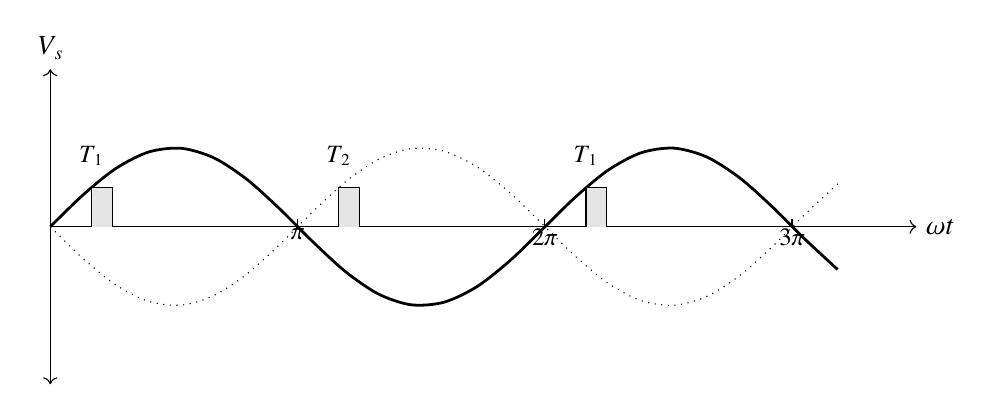
\begin{tikzpicture}[scale=1]
    \draw[->] (0,0) -- (11,0) node[right] {$\omega t$};
    \draw[<->] (0,-2) -- (0,2) node[above] {$V_s$};
    \draw[domain=0:10, smooth, variable=\x, black,line width=1pt] plot ({\x},{sin(deg(\x))});
    \draw[dotted,domain=0:10, smooth, variable=\x, black] plot ({\x},{-sin(deg(\x))});
    \foreach \x/\xtext in {3.14/\pi,6.28/2\pi,9.42/3\pi} {
        \draw (\x cm,0) -- (\x cm,0.1) node[below] {\small$\xtext$};
    }

\fill[gray!20] (0.5233,0) -- (0.5233,0.5) -- (0.785,0.5) -- (0.785,0) -- cycle;
    \fill[gray!20] (3.6633,0) -- (3.6633,0.5) -- (3.925,0.5) -- (3.925,0) -- cycle;
    \fill[gray!20] (6.8033,0) -- (6.8033,0.5) -- (7.065,0.5) -- (7.065,0) -- cycle;

    \draw (0.5233,0) -- (0.5233,0.5);
    \draw (0.5233,0.5) -- (0.785,0.5);
    \draw (0.785,0.5) -- (0.785,0);

    \draw (3.6633,0) -- (3.6633,0.5);
    \draw (3.6633,0.5) -- (3.925,0.5);
    \draw (3.925,0.5) -- (3.925,0);

    \draw (6.8033,0) -- (6.8033,0.5);
    \draw (6.8033,0.5) -- (7.065,0.5);
    \draw (7.065,0.5) -- (7.065,0);


     \node at (0.5233,0.9) {\small$T_1$};
     \node at (3.6633,0.9) {\small$T_2$};
     \node at (6.8033,0.9) {\small$T_1$};
\end{tikzpicture}
\end{figure}
\begin{figure}[!h]
    \centering
    \begin{tikzpicture}[scale=1]
    \draw[->] (0,0) -- (11,0) node[right] {$\omega t$};
    \draw[<->] (0,-2) -- (0,2) node[above] {$V_o$};
    \draw[domain=0.5233:3.14, smooth, variable=\x, black,line width=1pt] plot ({\x},{sin(deg(\x))});
    \draw[domain=3.6633:6.28, smooth, variable=\x, black,line width=1pt] plot ({\x},{-sin(deg(\x))});
    \draw[domain=6.8033:9.42, smooth, variable=\x, black,line width=1pt] plot ({\x},{sin(deg(\x))});

    \foreach \x/\xtext in {0.5233/\alpha, 3.14/\pi,4/\pi + \alpha ,6.28/2\pi,7.2/2\pi + \alpha,9.42/3\pi}{
        \draw (\x cm,0) -- (\x cm,0) node[below] {\small $\xtext$};
    }

     \draw [line width=1pt](0,0)--(0.5233,0);
    \draw [line width=1pt](0.5233,0) -- (0.5233,0.5);
    \draw[line width=1pt](3.14,0)-- (3.6633,0);
    \draw[line width=1pt] (3.6633,0) -- (3.6633,0.5);
    \draw [line width=1pt](6.28,0)--(6.8033,0);
    \draw [line width=1pt](6.8033,0) -- (6.8033,0.5);

    \node at (0.25,0.6){\small$T_2$};
    \node at (0.25,0.2){\small$D_2$};
     \node at (3.4,0.6){\small$T_1$};
    \node at (3.4,0.2){\small$D_1$};
    \node at (6.4,0.6){\small$T_2$};
    \node at (6.4,0.2){\small$D_2$};

    \node at (1.57,0.4){\small $T_1D_2$};
    \node at (4.71,0.4){\small $T_2D_1$};
    
\end{tikzpicture}
\end{figure}
\begin{figure}[!h]
    \centering
    \begin{tikzpicture}[scale=1]
    \draw[->] (0,0) -- (11,0) node[right] {$\omega t$};
    \draw[<->] (0,-2) -- (0,2) node[above] {$i_{T_1}$};
   
    \foreach \x/\xtext in {0.5233/\alpha,4/\pi + \alpha,7.2/2\pi + \alpha,10/3\pi + \alpha}{
        \draw (\x cm,0) -- (\x cm,0) node[below] {\small $\xtext$};
    }
     \draw [line width=1pt](0,0)--(0.5233,0);
    \draw [line width=1pt](0.5233,0) -- (0.5233,1);
    \draw[line width=1pt](0.5233,1)-- (3.6633,1);
    \draw[line width=1pt] (3.6633,1) -- (3.6633,0);
    \draw[line width=1pt] (3.6633,0) -- (6.8033,0);
    \draw [line width=1pt](6.8033,0)--(6.8033,1);
    \draw [line width=1pt](6.8033,1) -- (9.948,1);
     \draw [line width=1pt] (9.948,1) -- (9.948,0);

     \draw[dotted,domain=0:10, smooth, variable=\x, black] plot ({\x},{1});
     \node at (0.4,1.2) {\small $I_{DC}$};
\end{tikzpicture}
\end{figure}
\begin{figure}[!h]
    \centering
    \begin{tikzpicture}[scale=1]
    \draw[->] (0,0) -- (11,0) node[right] {$\omega t$};
    \draw[<->] (0,-2) -- (0,2) node[above] {$i_{s}$};
   

    \draw [line width=1pt](0.5233,0) -- (0.5233,1);
    \draw[line width=1pt](0.5233,1)-- (3.14,1);
    \draw[line width=1pt](3.14,1)-- (3.14,0);
    \draw[line width=1pt] (3.14,0) -- (3.6633,0);
    \draw[line width=1pt] (3.6633,0) -- (3.6633,-1);
    \draw[line width=1pt] (3.6633,-1) -- (6.28,-1);
    \draw[line width=1pt]  (6.28,-1) -- (6.28,0);
    \draw[line width=1pt] (6.28,0) -- (6.8033,0);
    \draw [line width=1pt](6.8033,0)--(6.8033,1);
    \draw [line width=1pt](6.8033,1) -- (9.42,1);
     \draw [line width=1pt] (9.42,1) -- (9.42,0);
     \draw [line width=1pt] (9.42,0) -- (9.948,0);

     \draw[dotted,domain=0:10, smooth, variable=\x, black] plot ({\x},{1});
     \node at (0.4,1.2) {\small $I_{DC}$};
    
\end{tikzpicture}
\end{figure}

From \tabref{tab:inputs.EE.59.2022}:
\begin{align}
   (I_{s_1})_{peak} &= \frac{4I_{dc}}{\pi}\cos{\left(\frac{\alpha}{2}\right)}\\
    &= \frac{4 \times 15 }{\pi}\times \cos{\frac{45 \degree}{2}}\\
    &=17.64 A 
\end{align}

%\end{document}

\newpage
\end{enumerate}
